% Basic stuff
\documentclass[a4paper,10pt]{article}
\usepackage[utf8]{inputenc}
\usepackage[nswissgerman]{babel}
\usepackage{scrextend}
\usepackage{lipsum}
\usepackage{amsmath}
\usepackage{gauss}
\usepackage{amssymb} % to import \leadsto

% 3 column landscape layout with fewer margins
\usepackage[landscape, left=0.75cm, top=1cm, right=0.75cm, bottom=1.5cm, footskip=15pt]{geometry}
\usepackage{flowfram}
\usepackage{floatrow}
\usepackage{amsmath}

\changefontsizes[8pt]{8pt}
\ffvadjustfalse
\setlength{\columnsep}{1cm}
\Ncolumn{3}

% define nice looking boxes
\usepackage[most]{tcolorbox}

% a base set, that is then customised
\tcbset {
  base/.style={
    boxrule=0mm,
    leftrule=1mm,
    left=1.75mm,
    arc=0mm, 
    fonttitle=\bfseries, 
    colbacktitle=black!10!white, 
    coltitle=black, 
    toptitle=0.75mm, 
    bottomtitle=0.25mm,
    title={#1}
  }
}

\definecolor{brandblue}{rgb}{0.34, 0.7, 1}
\newtcolorbox{mainbox}[1]{
  colframe=brandblue, 
  base={#1}
}

\newtcolorbox{subbox}[1]{
  colframe=black!20!white,
  base={#1}
}

% Mathematical typesetting & symbols
\usepackage{amsthm, mathtools, amssymb} 
\usepackage{marvosym, wasysym}
\allowdisplaybreaks

% Tables
\usepackage{tabularx, multirow}
\usepackage{booktabs}
\renewcommand*{\arraystretch}{2}

% Make enumerations more compact
\usepackage{enumitem}
\setitemize{itemsep=0.5pt}
\setenumerate{itemsep=0.75pt}

% To include sketches & PDFs
\usepackage{graphicx}

% For hyperlinks
\usepackage{hyperref}
\hypersetup{
  colorlinks=true
}

% Metadata
\title{Cheatsheet Lineare Algebra}
\author{Thomas Gassmann}
\date{August 2022}

% Math helper stuff
\def\limn{\lim_{n\to \infty}}
\def\limxo{\lim_{x\to 0}}
\def\limxi{\lim_{x\to\infty}}
\def\limxn{\lim_{x\to-\infty}}
\def\sumk{\sum_{k=1}^\infty}
\def\sumn{\sum_{n=0}^\infty}
\def\R{\mathbb{R}}
\def\dx{\text{ d}x}

\newcommand{\overbar}[1]{\mkern 1.5mu\overline{\mkern-1.5mu#1\mkern-1.5mu}\mkern 1.5mu}

\begin{document}

\begin{center}
  Lizenziert unter CC BY-SA 4.0. Für Urheber, Quellen und Lizenzinformationen, siehe:\\
  \href{https://github.com/thomasgassmann/eth-summaries}{thomasgassmann/eth-summaries}
\end{center}

\section{Vorwissen}
\subsection{Komplexe Zahlen}
\begin{mainbox}{Definition}
Ein Ausdruck der Form $z = a + ib$, wobei $i^2 = -1$. $a = Re(z)$ ist der Realteil, $b = Im(z)$ ist der Imaginärteil.
\end{mainbox}

Addition erfolgt komponentenweise, Multiplikation erfolgt unter Annahme des Binomialgesetzes und $i^2 = -1$ (i.e. $z w = (a c - b d) + i (a d + b  c)$). Für Division gilt $\frac{z}{w} = \frac{c + id}{a + ib} = \frac{(ca + bd) + i(ad - cb)}{a^2 + b^2}$.\\
Die Norm ist definiert als $|z| = \sqrt{Re(z)^2 + Im(z)^2} = \sqrt{z \cdot \overbar{z}}$. Für $z = x + iy$ ist $\overbar{z} = x - iy$ konjugiert-komplex.

\begin{subbox}{}
$$z \overbar{z} = Re(z)^2 + Im(z)^2$$
\end{subbox}

Eine komplexe Zahl kann in Polarkoordinaten dargestellt werden. Es gilt $z = re^{i\phi} = r(\cos(\phi) + i\sin(\phi))$.

\section{LGS / Gauss}

\begin{enumerate}
  \item Wir können Zeilen austauschen, eine Zeile mit $a \in \mathbb{R}\setminus \{0\}$ multiplizieren und Zeilen voneinander subtrahieren bzw. addieren.
  \item Wir schreiben das lineare Gleichungssystem (LGS) in Matrixform.
  \item Wir transformieren das LGS in die Zeilenstufenform.
  \item Wir lösen das LGS von unten nach oben.
\end{enumerate}



\section{Tabellen}

\begin{mainbox}{Wichtige Werte}
  \begin{center} 
   \begin{tabular}{c|cccccc}
    deg & 0° & 30° & 45° & 60° & 90° & 180° \\
    \midrule
    rad & 0 & $\frac{\pi}{6}$ & $\frac{\pi}{4}$ & $\frac{\pi}{3}$ & $\frac{\pi}{2}$ & $\pi$ \\
    cos & 1 & $\frac{\sqrt{3}}{2}$ & $\frac{\sqrt{2}}{2}$ & $\frac{1}{2}$ & 0 & -1 \\
    sin & 0 & $\frac{1}{2}$ & $\frac{\sqrt{2}}{2}$ & $\frac{\sqrt{3}}{2}$ & 1 & 0 \\
    tan & 0 & $\frac{1}{\sqrt{3}}$ & 1 & $\sqrt{3}$ & $+\infty$ & 0 \\
   \end{tabular}
  \end{center}
\end{mainbox}

\begin{center}
  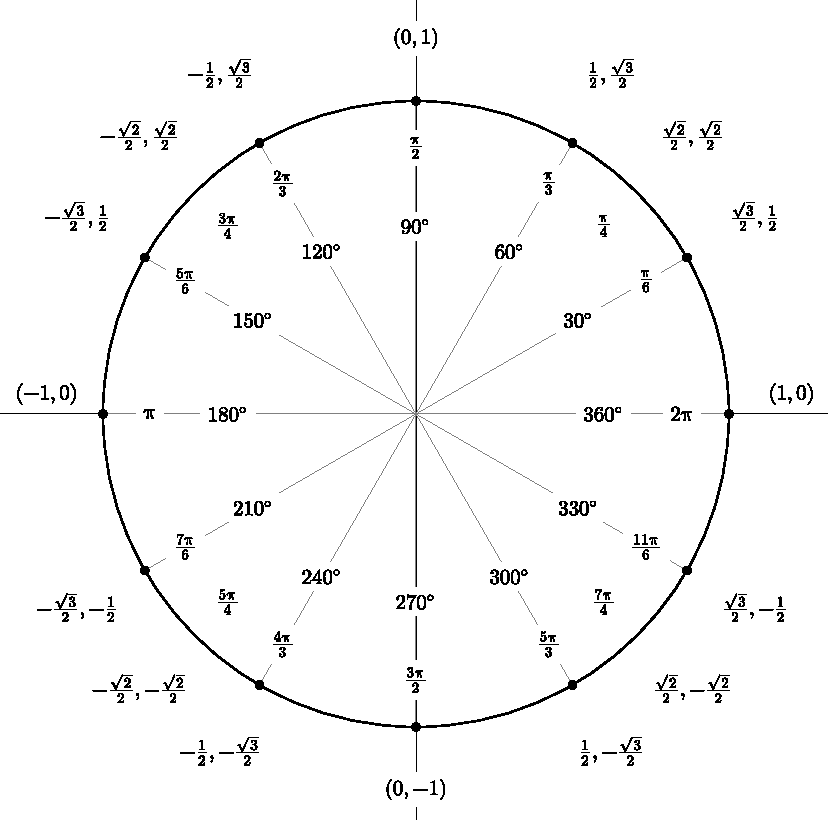
\includegraphics[width=\linewidth]{degrees_circle.pdf}
\end{center}

\end{document}
